\chapter{Realidade Aumentada}
\label{chapter:principios_ra}



A Realidade Aumentada aprimora a percepção do mundo pelo usuário, além de
lhe permitir interagir com essa realidade. Os objetos virtuais podem 
exibir informações que os usuários não detectariam diretamente sozinhos.
Esses dados podem ajudar os usuários a realizar tarefas reais do dia-a-dia
\cite{SurveyAR}.


Um dos principais pesquisadores sobre Realidade Aumentada nos últimos 20 anos
é o Ronald T. Azuma, Ph.D. Segundo ele, toda aplicação de Realidade Aumentada deve possuir
as seguintes características \cite{SurveyAR}:


% Azuma não detalha estes tópicos, por isso não foram melhores descritos aqui
\begin{enumerate}
    \item Combinação dos mundos real e virtual
    \item Interatividade em tempo real
    \item Sobreposição de objetos virtuais em 3D
\end{enumerate}







\section{Realidade Virtual e Realidade Aumentada}

A Realidade Aumentada é uma área derivada da Realidade Virtual, com distinções,
vantagens e desvantagens para determinados tipos de aplicações. Nas subseções 
seguintes serão abordadas essas características.


\subsection{Realidade Virtual}


Diversas aplicações, como tratamento de doenças e fobias, simulação de exames
médicos e procedimentos cirúrgicos, além de técnicas de extração de petróleo
podem ser beneficiadas com o uso da Realidade Virtual \cite{ARColaborativa}.


A Realidade Virtual é uma técnica que viabiliza a interação de elementos reais em ambientes
virtuais, gerados por computação. 
Um bom exemplo de Realidade Virtual são os simuladores de voo, simuladores de corrida etc, usados
por muitos pilotos durante treinamento e preparação.
Dessa forma, a Realidade Virtual é a completa imersão do usuário em um ambiente totalmente
gerado computacionalmente. A interação do usuário com esse ambiente é feita por meio de capacetes,
luvas ou outros equipamentos que permitam a transmissão de informações de movimentos e ações 
do usuário ao computador \cite{ARColaborativa}.

A Figura \ref{fig:equipamentos_rv} exibe alguns exemplos de equipamentos utilizados na Realidade
Virtual, para permitir a interação do usuário com a realidade gerada pela aplicação.

\begin{figure}[h!]
    \centering
    \caption{Exemplo de Equipamentos utilizados na Realidade Virtual}
    \label{fig:equipamentos_rv}
    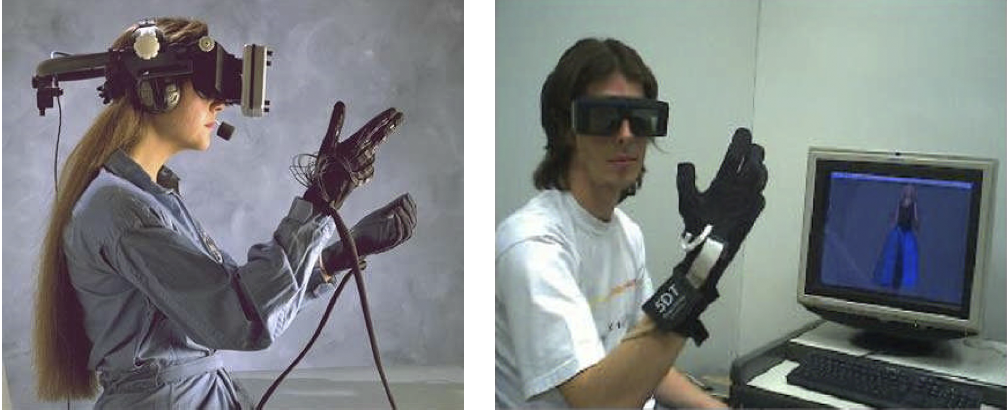
\includegraphics[width=14cm]{resources/equipamentos-rv.png}
\end{figure}



\subsection{Realidade Aumentada}


A Realidade Aumentada consiste na sobreposição de informações (imagens, textos e outros dados) a imagens
do mundo real, geralmente obtidas a partir de câmeras. Muitas aplicações estão usando a Realidade Aumentada
para prover maior interação entre o usuário e as informações ao seu redor. Um exemplo de aplicação da 
Realidade Aumentada é a sobreposição do fluxo sanguíneo em uma imagem dos vasos sanguíneos de um paciente,
obtida a partir de um exame médico \cite{ARColaborativa}.

A Figura \ref{fig:AR-map-locations11} mostra um exemplo de aplicação de Realidade Aumentada para geolocalização.

\begin{figure}[h!]
    \centering
    \caption{Exemplo de Realidade Aumentada para localização}
    \label{fig:AR-map-locations11}
    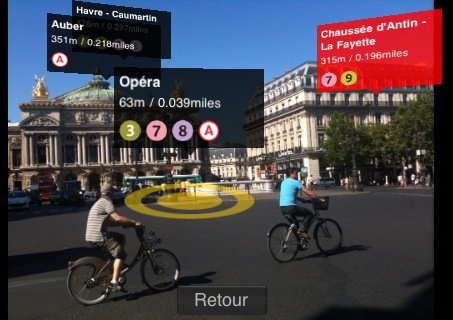
\includegraphics[width=15cm]{resources/augmented-reality-paris.jpg}
\end{figure}



\subsection{Diferenças entre Realidade Virtual e Realidade Aumentada}

A principal diferença entre Realidade Virtual e Realidade Aumentada
é que a primeira cria uma nova realidade ao usuário, com objetos
próprios, todos criados pela computação. Já a Realidade Aumentada
sobrepõe objetos virtuais a imagens da realidade humana, geralmente
captadas por câmeras digitais \cite{ARCADE, TrendsInAR}.
Segundo \cite{SurveyAR, AdvancesAR}, a Realidade Aumentada é
um suplemento à realidade, não uma substituição dela, de forma que,
para o usuário, a realidade e os objetos virtuais coexistem no mesmo
espaço. A Realidade Aumentada exige muita precisão na detecção da
localização e da posição do usuário, para que seja possível fornecer
uma interface com o usuário poderosa, por exemplo, mostrando objetos
virtuais baseados na posição e na direção para onde o usuário está
voltado.

Em determinados tipo de aplicação, a Realidade Aumentada pode prover maiores vantagens em 
relação à Realidade Virtual, dentre elas \cite{ARFeatureMaching}:

\begin{itemize}
    \item \textbf{A Realidade Aumentada provê melhor senso de realidade}\\
    
    A Realidade Virtual simula o mundo real por meio da computação, dando a
    sensação de imersão ao usuário. Por outro lado, a Realidade Aumentada 
    é uma integração do mundo real com o ambiente virtual, o que dá mais senso
    de realidade aos usuários.
    
    \item \textbf{A Realidade Aumentada permite maior interatividade}\\
    
    Como a Realidade Virtual enfatiza o mundo virtual como sendo seu principal
    recurso, o usuário permanece em situação passiva. Contudo, a Realidade Aumentada
    considera fundamental a integração entre mundo real e objetos virtuais. Assim,
    a Realidade Aumentada permite que os usuários participem e interajam com ela.
\end{itemize}

A Tabela \ref{tab:dif_AR_VR} mostra as principais diferenças entre
Realidade Virtual e Realidade Aumentada.

\begin{table}{h!}
    \centering
    \caption{Principais Diferenças entre Realidade Virtual e Realidade Aumentada}
    \label{tab:dif_AR_VR}
    \begin{tabular}{| p{5cm} | p{5cm} | p{5cm} |}
         \hline
         & Realidade Virtual & Realidade Aumentada \\
         \hline
         Ambiente Principal & Gerado por computador & Mundo real \\
         \hline
         Sentido da Presença & Controlado por computador & Natural do usuário \\
         \hline
         Impacto da transição do mundo real para o virtual & Alta & Baixa \\
         \hline
         Representação do usuário & Através de um avatar & Direta \\
         \hline
    \end{tabular}
\end{table}

Pesquisas anteriores por \cite{AppsHandheldDevices} e \cite{FieldTrips}
concluíram que a combinação de detecção de localização do usuário e
abordagem de aprendizado contextual pode facilitar a construção de 
conceitos mais precisos por usuários dessas tecnologias.

O foco principal deste trabalho é a Realidade Aumentada, por ser mais adequada 
à aplicação proposta. Por se tratar de uma aplicação de geolocalização, o usuário
não pode ter a sensação de imersão em uma realidade criada computacionalmente. É
imprescindível que a realidade do usuário não seja alterada, apenas complementada 
com informações relevantes.






\section{Realidade Aumentada em Dispositivos Móveis}
\label{sec:ra_mobile}

O uso de dispositivos móveis vem aumentando muito rapidamente nos últimos anos.
Segundo a \textit{Strategy Analytics}
\footnote{\href{http://www.strategyanalytics.com}{http://www.strategyanalytics.com}},
em outubro de 2012, a quantidade de \textit{smartphones} no mundo ultrapassou a faixa
de 1 bilhão. Desse total, apenas no período entre setembro de 2011 a outubro de 2012, 
a soma foi de 330 milhões de novos dipositivos e 79 milhões no segundo quadrimestre de 2012.
Segundo essa mesma pesquisa, nos próximos 3 anos será atingida a marca de 2 bilhões de
\textit{smartphones}.


Até recentemente, a Realidade Aumentada era utilizada predominantemente 
em \textit{desktops} e em ambientes virtuais. Porém, \cite{SurveyAR}
considerou que um sistema de Realidade Aumentada ideal deveria 
funcionar em qualquer ambiente natural, sem limitação de alcance e sem prévio
conhecimento do local onde o sistema atuará.

A Realidade Aumentada Móvel (\textit{Mobile Augmented Reality}) foi criada e estudada
antes mesmo da criação dos dispositivos móveis atuais, como \textit{smartphones} e 
\textit{tablets} \cite{ExperiencesWithHandheldAR, HouseOfOlbrich}. Os pesquisadores acoplavam câmeras a
telas de computadores reduzidos, que possuíam um dispositivo de saída (\textit{display}),
onde eram exibidas as imagens para o usuário, após serem processadas pelo programa. 
Todo esse processo deveria ocorrer em tempo real, de forma a permitir ao usuário a interação
com o ambiente.



Os usuários de dispositivos móveis os utilizam para diversos objetivos, não somente para fazer
ligações, navegar na Internet ou verificar suas caixas de email. Uma das principais utilidades
dos \textit{smartphones} é para localização, via \gls{GPS}. Há muitas aplicações de mapas, 
com imagens provenientes 
de satélites etc, que facilitam a vida dos usuários, principalmente em viagens para locais não
conhecidos. Seguindo a mesma ideia de localização, é possível criar aplicações específicas para
esse fim, focadas em áreas menores e mais específicas, auxiliando o usuário a se localizar, por exemplo, dentro
de um campus de um Universidade, no interior de um museu \cite{ARMuseumGuide} ou mesmo em uma
visita a um local turístico ou histórico \cite{HouseOfOlbrich}. 
Como se tratam de áreas mais restritas, a visualização de mapa, nestes casos, torna-se
menos adequada, por não exibir detalhes suficientes do local. Uma alternativa viável é utilizar as 
imagens captadas pelas próprias câmeras dos \textit{smartphones}: em vez de mapas de satélites com marcadores
para assinalar os locais conhecidos, é possível usar a Realidade Aumentada para exibir a localização dos
locais conhecidos. Dessa forma, conforme o usuário se move no ambiente, os marcadores dos locais conhecidos são
deslocados na tela, mostrando exatamente para onde o usuário deve seguir a fim de chegar ao seu destino 
\cite{MOOAR, MOOAR_Study}.

Devido a todos esses avanços, o uso de aplicações de Realidade Aumentada, exibindo informações relacionadas aos objetos
ao redor do usuário, vem crescendo muito \cite{BooksOnAShelf}. As aplicações mais comuns utilizam imagens capturadas pelas câmeras
dos dispositivos, localização via \gls{GPS} e orientação do equipamento provenientes dos dados de bússola e giroscópio,
presentes na maioria
dos \textit{smartphones} atuais, para criar camadas de dados relevantes para o usuário, conforme sua localização e sua orientação.


A Figura \ref{fig:AR-map-locations12} mostra um exemplo de aplicações de Realidade
Aumentada para localização de pontos de interesse.

\begin{figure}[h!]
    \centering
    \caption{Exemplo de Realidade Aumentada Móvel para localização}
    \label{fig:AR-map-locations12}
    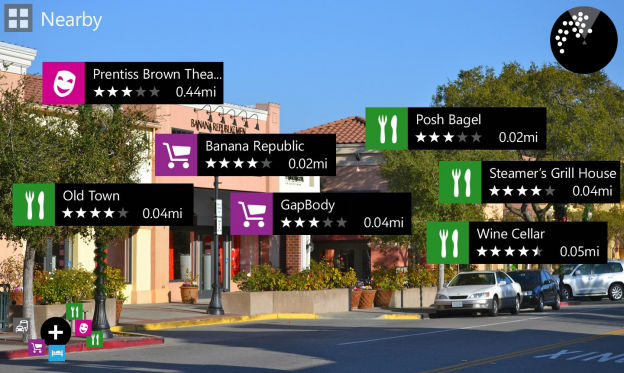
\includegraphics[width=15cm]{resources/nokia_city_lens-625x373-c.png}
\end{figure}




\label{def:hmd}
Muitas vezes, para exibição das informações, são usadas telas acopladas a capacetes,
chamadas \gls{HMD}. O \gls{HMD} consiste em um dispositivo acomodado na cabeça, de forma a cobrir os olhos.
Esses capacetes possuem uma tela onde são exibidas as imagens após seus processamentos pelo computador
responsável por criar a aplicação de Realidade Virtual ou de Realidade Aumentada. Também é possível
fornecer fones de ouvido ao usuário, para aumentar a imersão dele no mundo virtual gerado pelo sistema.
A Figura \ref{fig:hmd_example} mostra alguns tipos de \gls{HMD},

\begin{figure}[h!]
    \centering
    \caption{Exemplos de HDM (Head Mounted Display)}
    \label{fig:hmd_example}
    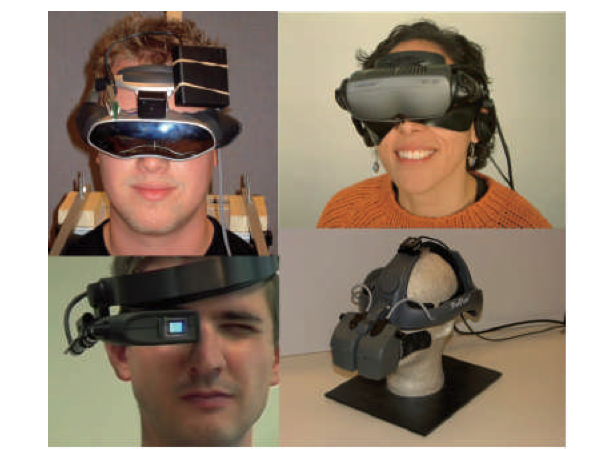
\includegraphics[width=13cm]{resources/HMD.png}
\end{figure}


Outra aplicação muito utilizada em Realidade Aumentada Móvel é o reconhecimento de códigos de barras e códigos QR
(\textit{QR Code}). Os códigos de barras comuns permitem detectar apenas dados numéricos, com o auxílio de um
leitor adequado (\textit{scanner}). Os Códigos QR (\textit{QR Code}, do inglês \textit{Quick Response}) podem 
representar dados alfanuméricos, permitindo descrever diversos outros tipos de dados, como número de telefone,
endereços de e-email e de \textit{web sites}, além de pequenos textos \cite{QRCodeSite}. A Figura 
\ref{fig:codigos-barras-qr-code} ilustra, do lado esquerdo, um código de barras comum e, do lado direito, um 
código QR.

\begin{figure}[h!]
    \centering
    \caption{Códigos de barras, usados em muitas aplicações de Realidade Aumentada Móvel}
    \label{fig:codigos-barras-qr-code}
    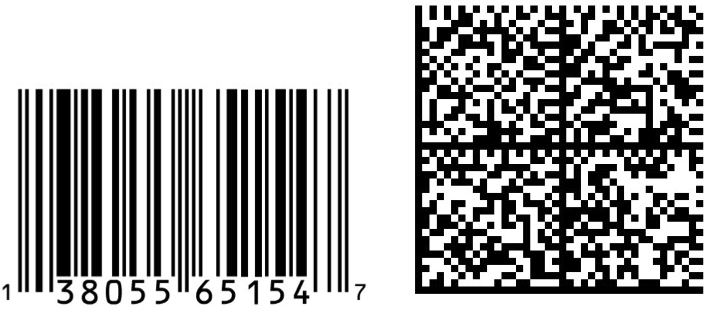
\includegraphics[width=13cm]{resources/codigo-barras-qr-code.png}
\end{figure}


\cite{HandheldAR} escreveu uma dos mais completos trabalhos sobre Realidade Aumentada para
dispositivos móveis. Além de vários detalhes técnicos, como rastreamento de objetos sem marcadores 
(\textit{markless tracking}) em dispositivos móveis, diversos casos de uso são descritos, demonstrando
a aplicabilidade da Realidade Aumentada Móvel.



\section{Técnicas da Realidade Aumentada}

A Realidade Aumentada envolve sensores (como \gls{GPS} e bússola), visão computacional,
interação humano-computador, realidade virtual e muitas outras áreas do conhecimento.
As principais tecnologias da Realidade Aumentada incluem visualização (\textit{display}),
\textit{registration}, \textit{tracking} e interatividade \cite{ARFeatureMaching}.



\subsection{\textit{Tracking}}

O processo chamado de \textit{Tracking}, ou \textbf{rastreamento}, consiste na detecção da posição e da direção
do usuário. 


Em geral, sistemas de Realidade Aumentada projetados para uso externo baseiam-se em localização
utilizando \gls{GPS}, orientação magnética (bússola) e sensores de inércia para determinar a 
orientação do usuário no espaço tridimensional. 

De 1998 até 2008, a técnica de \textit{Tracking} foi o tema mais recorrente em pesquisas científicas
\cite{TrendsInAR}. Isso mostra como ela é essencial para o desenvolvimento e para o
aprimoramento das aplicações utilizando Realidade Aumentada.


Há três categorias de \textit{Tracking}: 1) \textit{Tracking} Baseada em Sensores,
2) \textit{Tracking} Baseada em Visão Computacional e 3) \textit{Tracking} Híbrida.

Além disso, existem duas formas principais de fazer rastreamento (\textit{tracking}): utilizando
marcadores e não os utilizando (\textit{markerless}). A primeira categoria é utilizada
predominantemente em rastreamento por visão computacional, enquanto a segunda está mais ligada
a rastreamento por sensores. Ambas essas técnicas serão discutidas com mais detalhes a seguir.




\subsubsection{Tracking Baseado em Sensores}

Esta técnica pode se basear em sensores magnéticos, acústicos, 
de inércia, óptico e mecânico. Todos eles possuem suas vantagens
e desvantagens. Por exemplo, sensores magnéticos possuem alta frequência de atualização,
mas são facilmente afetados por qualquer material metálico próximo que altere o campo 
magnético da região analisada. 

Essa categoria de \textit{Tracking} foi desenvolvida no final da década de 1990, e apresentada
no \textbf{IWAR}
\footnote{International Workshop on Augmented Reality} 
de 1998. Desde então, pesquisadores estão estudando maneiras de combinar diversos
sensores, a fim de obter resultados mais fiéis e confiáveis.


\subsubsection{Tracking Baseado em Visão Computacional}

Esta técnica utiliza processamento de imagens para calcular a posição do usuário no espaço. 
É a categoria de \textit{tracking} com mais pesquisas no \textbf{ISMAR}
\footnote{International Symposium on Mixed and Augmented Reality}, 
de 1998 a 2008, com mais
de 80\% de presença em artigos científicos publicados nesse simpósio.

Esse método é um dos mais conhecidos e usados em Visão Computacional, em se tratando de
\textit{tracking} com marcadores. Ele consiste em
colocar marcadores fixos no ambiente, reconhecê-los por meio de Visão Computacional, e,
por fim, calcular a posição e a direção da câmera, a partir dos resultados da etapa anterior.
A Figura \ref{fig:AR-marker} ilustra o processo de reconhecimento de marcadores nesta
técnica de rastreamento. A Figura \ref{fig:AR-marker-example1} apresenta um exemplo de aplicação
usando rastreamento (\textit{tracking}) baseado em marcadores.

\begin{figure}[h!]
    \centering
    \caption{Reconhecimento de marcadores no processo de rastreamento (\textit{tracking})}
    \label{fig:AR-marker}
    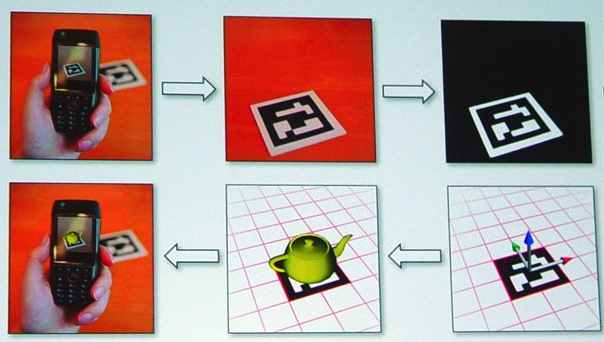
\includegraphics[width=15cm]{resources/marker-tracking.jpg}
\end{figure}



\begin{figure}[h!]
    \centering
    \caption{Exemplo de aplicação com rastreamento (\textit{tracking}) usando marcadores}
    \label{fig:AR-marker-example1}
    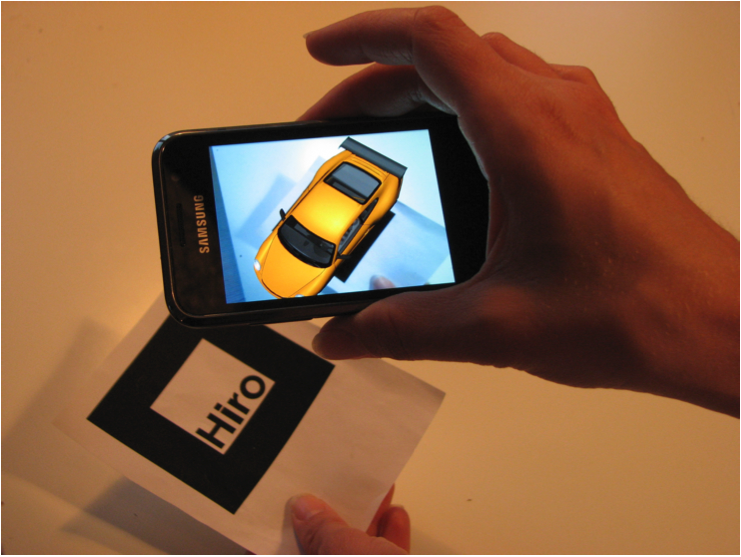
\includegraphics[width=15cm]{resources/marker-tracking-example1.png}
\end{figure}



\label{def:6dof}
Um dos conceitos explorados neste tipo de rastreamento é o \gls{6DOF},
que consiste na obtenção, por meio de sensores como acelerômetro e giroscópio, 
dos seis valores de posicionamento e orientação do dispositivo no espaço
tridimensional: três posições de rotação e três de translação. A Figura 
\ref{fig:6dof_data} mostra os seis dados relacionados com o \gls{6DOF}.

\begin{figure}[h!]
    \centering
    \caption{Os seis graus de liberdade (6DOF)}
    \label{fig:6dof_data}
    %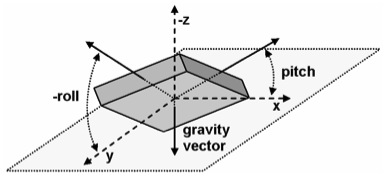
\includegraphics[width=15cm]{resources/6DOF.png}
    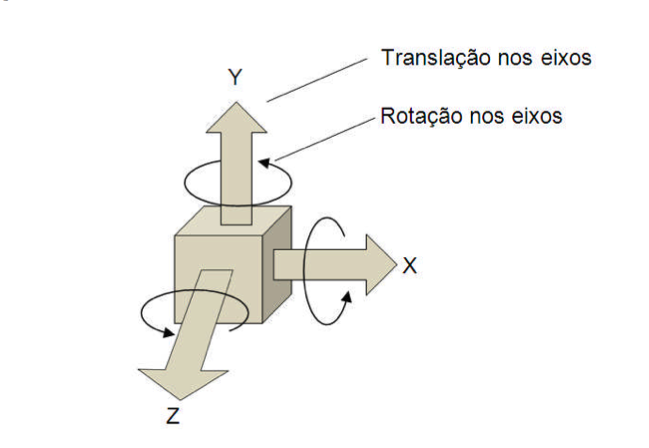
\includegraphics[width=15cm]{resources/6DoF-ptbr.png}
\end{figure}



O \textit{tracking} baseado em visão computacional busca associar traços de imagens 
digitais 2D em coordenadas no mundo real, em 3D.
A posição da câmera pode ser obtida projetando-se as coordenadas 3D nas coordenadas
da imagem 2D observada.    



\subsubsection{Tracking Híbrido}

Considerando que cada técnica citada anteriormente possui vantagens e desvantagens, 
foi proposta a combinação entre algumas delas. Por exemplo, Azuma\cite{SurveyAR}
propôs um sistema de Realidade Aumentada para uso externo que utiliza \gls{GPS}, 
sensores de inércia e visão computacional.

Em \cite{HybridTrackingOutdoorAR}, é abordado o desenvolvimento de um modelo de \textit{tracking}
híbrido, em que é utilizado um giroscópio (\textit{tracking} baseado em sensores)
e visão computacional.

O artigo \cite{HybridTrackingForGIS} também descreve uma técnica de \textit{tracking} híbrido,
em que são utilizadas informações de \gls{GPS} e de sensores de inércia para obter a localização,
a posição e a orientação do usuário no espaço.







\subsection{\textit{Registration}}

O processo chamado de \textit{Registration} consiste na sobreposição de objetos
virtuais às imagens da realidade. Esse método é fundamental para a garantia
de desempenho do sistema de Realidade Aumentada. Esse também é um dos principais
temas de pesquisa da Realidade Aumentada \cite{DevActuallyRegistration}.

O \textit{Registration} é um processo complexo, principalmente em aplicações de
Realidade Aumentada para uso externo (\textit{outdoor}). Ao se projetar um
sistema de Realidade Aumentada para uso externo, requisitos especiais de
equipamentos e de modelo de aplicação devem ser considerados. Em geral, eles
têm características de mobilidade, multi-dimensão e tempo real \cite{DevActuallyRegistration}.


O processo de \textit{Registration} também é crucial em muitas aplicações para uso interno
(\textit{indoor}). Imagine uma aplicação de Realidade Aumentada para uso médico, para biópsias.
Se o objeto virtual não estiver no local exato onde o verdadeiro tumor está, a agulha não atingirá
o local adequado e a biópsia falhará. Sem um processo de \textit{Registration} apurado e preciso, 
a Realidade Aumentada pode não ser aceitável em muitos tipos de aplicações, como a citada acima 
\cite{SurveyAR}.






Classifica-se o processo de \textit{Registration} em três grupos: 1) baseada em
rastreamento (\textit{tracker-based registration}), 2) baseada em conhecimento
(\textit{knowledge-based registration}) e 3) baseada em visão computacional
(\textit{computer vision-based registration}) \cite{DevActuallyRegistration}.



\subsubsection{Baseada em Rastreamento (\textit{Tracker-based Registration})}


O processo de \textit{Registration} baseado em rastreamento inclui: mecânica,
sensores magnéticos, GPS, ultrasonicos, inércia e óptica. A Tablea \ref{tab:track-reg-comp}
compara cada uma dessas técnicas.

\begin{table}[h!]
    \caption{Comparação entre técnicas de \textit{Registration}}
    \label{tab:track-reg-comp}
    \begin{tabular}{| p{5cm} | p{5cm} | p{5cm} |}
        \hline
        Tecnologia de \textit{Tracking} & Vantagens & Desvantagens \\
        \hline
        Mecânica & Exatidão, baixo atraso no processamento, sem influência visual ou magnética, fácil rastreamento de objetos pequenos & Uso limitado \\
        \hline
        Sensores Magnéticos & baixo preço, exatidão, sem interferências visuais, imune a sons, eficiente mesmo em áreas amplas & Facilmente influenciada por campos magnéticos e presença de metais no ambiente \\
        \hline
        GPS & ideal para áreas amplas & falta de precisão e atraso no processamento \\
        \hline
        Ultrasônico & baixo preço, sem influência de campos magnéticos, baixo uso de equipamentos & facilmente distorcida no ambiente, baixa precisão a grandes distâncias \\
        \hline
        Inércia & sem limitação de distâncias, alta velocidade, sem influência de visão ou campo magnético, tamanho pequeno e baixo custo & apenas 3 graus de liberdade\footnote{\textit{3 Degrees Of Freedom}: apenas 3 dos 6 possíveis graus de liberdade}, espalhamento e baixa precisão em altas velocidades \\
        \hline
    \end{tabular}
\end{table}




\subsubsection{Baseado em Conhecimento (\textit{Knowledge-based})}


O processo de \textit{Registration} Baseado em Conhecimento (\textit{Knowledge-based}) foi
proposto pelo Laboratório de Interface de Usuários, do Departamento de Ciência da Computação, 
da Universidade de Columbia, durante o desenvolvimento de um projeto de Realidade Aumentada.
Os rastreadores são fixados em equipamentos de formato conhecido, de forma a garantir a posição
e a orientação. O maior problema desse método é a necessidade de conhecer a estrutura dos equipamentos,
além de haver atraso e erros entre os rastreadores.



\subsubsection{Baseado em Visão Computacional (\textit{Computer vision-based})}

Devido à fácil teorização e à conveniência na realização, o \textit{registration} basedo em visão computacional
vem sendo a técnica de maior potencial em aplicações de Realidade Aumentada. Em teoria, ele possui alta precisão,
podendo chegar ao nível de \textit{pixels}.

O \textit{registration} baseado em visão computacional pode ser separado em duas categorias: 1) baseado em
calibragem de câmera (\textit{camera calibration}) e 2) baseado em transformação afim
(\textit{affine transformation}).

\begin{enumerate}
    \item \textbf{Baseado em Calibragem de Câmera}
    
    Esta é a categoria mais comum de \textit{registration} baseada em visão computacional. 
    Este método coloca marcadores no ambiente, reconhece-os por meio de visão computacional e, com essas informações, 
    calcula a posição e a orientação onde os objetos virtuais devem ser posicionados. 


    \item \textbf{Baseado em Transformação Afim}
    
    Segundo \cite{AffineStructure}, se ao menos quatro pontos não-coplanares em um espaço 3D são conhecidos, 
    para toda transformação de projeção, o resultado da transformação de cada ponto pode ser representado por
    uma combinação linear de quatro pontos. Dessa forma, a Teoria da Transformação Afim é introduzida na 
    Realidade Aumentada e o complexo processo de calibragem é traduzido para o processo de posicionamento de
    projeções 2D de pontos no plano.
\end{enumerate}


\section{Realidade Aumentada \textit{Indoor} X \textit{Outdoor}}

Realidade Aumentada para ambientes internos (\textit{Indoor Augmented Reality})
geralmente utiliza \textit{tracking} baseada em marcadores, a fim de detectar
a direção para onde a câmera está apontando, ou mesmo qual objeto ela está
focalizando. Na Realidade Aumentada para ambientes externos (\textit{Outdoor Augmented Reality}),
é muito mais complexa a detecção da posição e da orientação do usuário. A utilização 
de marcadores torna-se muito mais complexa, devido ao tamanho da área abrangida pela aplicação.
Por isso, nesse tipo de Realidade Aumentada costuma-se usar \textit{tracking} baseado em sensores,
como \gls{GPS}, giroscópio e bússola, os quais permitem obter, com alta exatidão, a posição e a
orientação do usuário no espaço \cite{HybridTrackingForGIS}.





\section{Trabalhos Relacionados}
\label{sec:trab_relacionados}



Há diversos trabalhos relacionados a aplicações baseadas em Realidade
Aumentada \cite{MOOAR_Study}. 


Em \cite{HybridTrackingOutdoorAR}, é abordado o desenvolvimento de um modelo de \textit{tracking}
híbrido, em que é utilizado um giroscópio (\textit{tracking} baseado em sensores)
e visão computacional.


O artigo \cite{HybridTrackingForGIS} também descreve uma técnica de \textit{tracking} híbrido,
em que são utilizadas informações de \gls{GPS} e de sensores de inércia para obter a localização,
a posição e a orientação do usuário no espaço.


Um dos exemplos mais conhecidos atualmente é o \textit{Google Glass}
\footnote{\href{http://www.google.com/glass}{http://www.google.com/glass}}.
O Google Glass é um projeto do Google, com o objetivo de criar um óculos que exibe
informações para o usuário em \textit{displays} embutidos nas próprias lentes.

% No Museu de Ciência e Indústria (\textit{Museum of Science and Industry}), em Chicago,
% está exposta uma ferramenta de Realidade Aumentada que exibe, em uma mesa digital, a
% Tabela Periódica dos Elementos Químicos. Os usuários podem, arrastando um grupo de 
% elementos, criar simulações de reações químicas. A Figura \ref{fig:tabela-periodica-AR}
% ilustra essa ferramenta. O usuário pode arrastar dois ou mais elementos da Tabela
% Periódica para a área lateral direita da mesa, demarcada por uma circunferência, onde
% a simulação da reação ocorrerá.
% 
% 
% \begin{figure}[h!]
%     \centering
%     \caption{Aplicação de Realidade Aumentada do \textit{Museum of Science and Industry} para criar simulações de reações químicas}
%     \label{fig:tabela-periodica-AR}
%     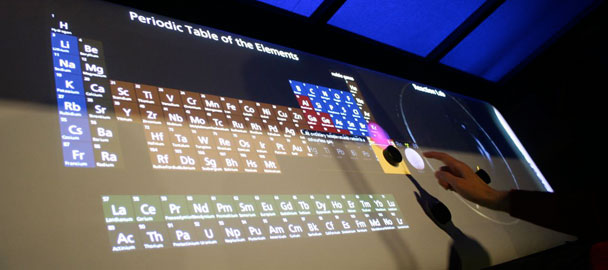
\includegraphics[width=14cm]{resources/tabela-periodica-AR.jpg}
% \end{figure}




Há, pelo menos, seis principais classes de aplicações de 
Realidade Aumentada exploradas até o momento: 1) médica, 2) manufatura e reparos,
3) anotações e visualização, 4) robótica, 5) entretenimento e 6) aplicações militares \cite{SurveyAR}.


\subsection{Área Médica}

Médicos podem utilizar a Realidade Aumentada como uma ferramenta de auxílio
no estudo e no treinamento para cirurgias e outros procedimentos. Várias 
aplicações estão explorando essa área. Na \textit{UNC Chapel Hill}, um grupo
de pesquisas coletou imagens do útero de mulheres grávidas usando ultrassonografia,
gerando uma representação 3D do feto dentro do útero e a exibindo em um \gls{HMD}, 
conforma a Figura \ref{fig:feto_utero_3d}. O objetivo é permitir ao médico analisar todos os movimentos
do feto dentro do útero, de forme que isso um dia torne-se uma espécie de estetoscópio 3D \cite{Feto3D}.

\begin{figure}[h!]
    \centering
    \caption{Imagem 3D de um feto dentro do útero (pesquisa da UNC Chapel Hill)}
    \label{fig:feto_utero_3d}
    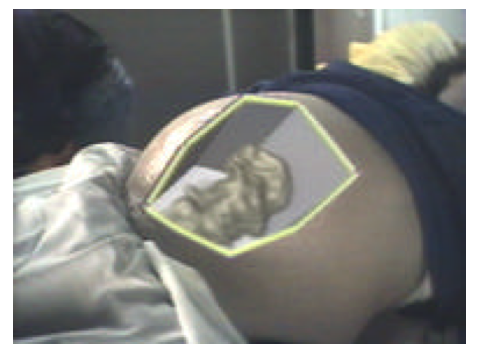
\includegraphics[width=10cm]{resources/feto-3d.png}
\end{figure}



\subsection{Manufatura e Reparos}

Outra aplicação para a Realidade Aumentada é na montagem, manutenção e reparo
de maquinários. Os procedimentos para essas atividades, em vez de estarem descritas
em texto na forma de manuais, poderia ser visualizada em 3D, sobrepostas aos
próprios equipamentos. É possível, inclusive, criar animações, mostrando exatamente
como proceder para realizar a tarefa. O grupo de Steve Feiner, em Columbia, desenvolveu
uma aplicação para manutenção de impressoras a \textit{laser} \cite{LaserPrinterAR}. 
A Figura \ref{:laser_printer_1} a visão externa a Figura \ref{:laser_printer_2} 
exibe a visão do usuário, onde uma 
imagem gerada por computador orienta o usuário a remover a bandeja de papel.


\begin{figure}[h!]
    \centering
    \caption{Visão externa do sistema de reparos de impressoras a laser}
    \label{fig:laser_printer_1}
    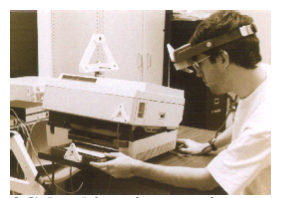
\includegraphics[width=10cm]{resources/laser-printer-1.png}
\end{figure}


\begin{figure}[h!]
    \centering
    \caption{Visão do usuário no sistema de reparos de impressoras a laser}
    \label{fig:laser_printer_2}
    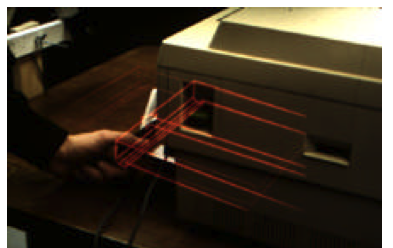
\includegraphics[width=10cm]{resources/laser-printer-2.png}
\end{figure}



\subsection{Anotação e Visualização}

Chang, W. \cite{MOOAR} propôs o
\textit{``Multi-Object Oriented Augmented Reality''} (MOOAR), também 
estudado por Chang and Tan em \cite{MOOAR_Study}. O \textit{MOOAR} foi
proposto para ambientes de aprendizado baseado em localização. Sua
implementação usa a Realidade Aumentada como principal ferramenta para
prover conteúdo interativo de aprendizado através de objetos virtuais.
O MOOAR visa a reduzir os desvios e aumentar a interação entre usuários,
objetos e conteúdo, a fim de melhorar a eficácia da aprendizagem.

Em \cite{AugmentedMaps} é proposta outra forma de Realidade Aumentada
baseada em mapas. Usando um mapa impresso como base, ao focar uma câmera sobre determinados
pontos do mapa, informações digitais eram sobrepostas à imagem, fornecendo maiores detalhes
ao usuário.



\subsection{Robótica}

Teleoperação de robôs é sempre uma tarefa complexa, especialmente quando o robô está distante, devido a falhas
na comunicação.Nessas condições, é preferível controlar um robô virtual, em vez do real. O operador planeja a 
rota do robô, guiando um robô virtual. Após traçado o trajeto, o robô real recebe as mesmas coordenadas recebidas
pelo virtual, o qual as segue, sem que haja erros ocasionados pela falha na comunicação entre o operador e o 
robô. Diversos autores criaram protótipos para essa finalidade \cite{RobotAR1,RobotAR2,RobotAR3}.


\subsection{Entretenimento}

A aplicação \textit{Archeoguide} \cite{Archeoguide} propôs uma viagem pelas ruínas de civilizações antigas usando
a Realidade Aumentada. O usuário visita a antiga Olympia, na Grécia, utilizando uma tela acoplada a um capacete
(\gls{HMD}), ligada a um computador semi-portátil, dentro de uma mochila. O sistema identifica 
artefatos e áreas danificadas, reconstruindo-as digitalmente na tela, e exibindo informações sobre os antigos 
esportes olímpicos. 

O projeto \textit{ALIVE}, do \textit{MIT Media Lab}, criou uma aplicação que adiciona ao ambiente
criaturas inteligentes virtuais, que reagem às ações dos usuários \cite{ArtificialLife}.





\subsection{Aplicações Militares}


A \textit{Boeing Computer Seattle} está desenvolvendo aplicações utilizando a Realidade Aumentada com o objetivo
de mostrar aos pilotos das aeronaves o maior número de informações relevantes sobre uma rota, ou mesmo auxiliá-los 
durante um combate. Já existem helicópteros que possuem um capacete para o piloto que está interligado com a mira 
de uma ou mais armas da aeronave. Dessa forma, para que o piloto mire o inimigo, basta olhar para ele \cite{ARCADE}.











